%% 
%% Copyright 2007-2020 Elsevier Ltd
%% 
%% This file is part of the 'Elsarticle Bundle'.
%% ---------------------------------------------
%% 
%% It may be distributed under the conditions of the LaTeX Project Public
%% License, either version 1.2 of this license or (at your option) any
%% later version.  The latest version of this license is in
%%    http://www.latex-project.org/lppl.txt
%% and version 1.2 or later is part of all distributions of LaTeX
%% version 1999/12/01 or later.
%% 
%% The list of all files belonging to the 'Elsarticle Bundle' is
%% given in the file `manifest.txt'.
%% 

%% Template article for Elsevier's document class `elsarticle'
%% with numbered style bibliographic references
%% SP 2008/03/01
%%
%% 
%%
%% $Id: elsarticle-template-num.tex 190 2020-11-23 11:12:32Z rishi $
%%
%%
\documentclass[preprint,12pt]{elsarticle}

\usepackage[dvipsnames]{xcolor}
%% Use the option review to obtain double line spacing
%% \documentclass[authoryear,preprint,review,12pt]{elsarticle}

%% Use the options 1p,twocolumn; 3p; 3p,twocolumn; 5p; or 5p,twocolumn
%% for a journal layout:
%% \documentclass[final,1p,times]{elsarticle}
%% \documentclass[final,1p,times,twocolumn]{elsarticle}
%% \documentclass[final,3p,times]{elsarticle}
%% \documentclass[final,3p,times,twocolumn]{elsarticle}
%% \documentclass[final,5p,times]{elsarticle}
%% \documentclass[final,5p,times,twocolumn]{elsarticle}

%% For including figures, graphicx.sty has been loaded in
%% elsarticle.cls. If you prefer to use the old commands
%% please give \usepackage{epsfig}

%% The amssymb package provides various useful mathematical symbols
\usepackage{amssymb,amsthm,amsmath}
%% The amsthm package provides extended theorem environments
%% \usepackage{amsthm}
% The float package adjusts figures' positioning
\usepackage{float}
% The mchem package adds support for displaying chemistry notations
\usepackage[version=4]{mhchem}
\usepackage{cleveref}

\usepackage{pifont}% http://ctan.org/pkg/pifont
\newcommand{\cmark}{\ding{51}}%
\newcommand{\xmark}{\ding{55}}%
% \usepackage[linesnumbered, algochapter, ruled, longend]{algorithm2e}
% \usepackage{cleveref}
% \usepackage{tabularx}
\usepackage{tikz}
\usetikzlibrary{positioning,fit,backgrounds,arrows.meta, calc, patterns}


%% The lineno packages adds line numbers. Start line numbering with
%% \begin{linenumbers}, end it with \end{linenumbers}. Or switch it on
%% for the whole article with \linenumbers.
%% \usepackage{lineno}

\journal{Tomography of Materials and Structures}

\begin{document}

\begin{frontmatter}

%% Title, authors and addresses

%% use the tnoteref command within \title for footnotes;
%% use the tnotetext command for theassociated footnote;
%% use the fnref command within \author or \address for footnotes;
%% use the fntext command for theassociated footnote;
%% use the corref command within \author for corresponding author footnotes;
%% use the cortext command for theassociated footnote;
%% use the ead command for the email address,
%% and the form \ead[url] for the home page:
%% \title{Title\tnoteref{label1}}
%% \tnotetext[label1]{}
%% \author{Name\corref{cor1}\fnref{label2}}
%% \ead{email address}
%% \ead[url]{home page}
%% \fntext[label2]{}
%% \cortext[cor1]{}
%% \affiliation{organization={},
%%             addressline={},
%%             city={},
%%             postcode={},
%%             state={},
%%             country={}}
%% \fntext[label3]{}

\title{Synthetic Particle Pack Generation for Augmentation and Testing in Geological Tomographic Segmentation}

%% use optional labels to link authors explicitly to addresses:
%% \author[label1,label2]{}
%% \affiliation[label1]{organization={},
%%             addressline={},
%%             city={},
%%             postcode={},
%%             state={},
%%             country={}}
%%
%% \affiliation[label2]{organization={},
%%             addressline={},
%%             city={},
%%             postcode={},
%%             state={},
%%             country={}}

\author[inst1]{Bogong Wang}
\author[inst2]{Andrew Kingston}
\author[inst2]{Philipp D. L\"{o}sel}
\author[inst1]{Warren Creemers}

\affiliation[inst1]{organization={School of Computing},%Department and Organization
            addressline={The Australian National University}, 
            city={Canberra},
            postcode={2617}, 
            state={ACT},
            country={Australia}}

\affiliation[inst2]{organization={Research School of Physics},%Department and Organization
            addressline={The Australian National University}, 
            city={Canberra},
            postcode={2617}, 
            state={ACT},
            country={Australia}}


\begin{abstract}
%% Text of abstract
3D imaging of geological particle samples by computed tomography (CT) offers the means for non-destructive analysis. 
However, obtaining such tomograms with the corresponding segmentation labels remains a significant challenge. 
% Current methods are constrained by the need for extensive manual inspection and correction, as the initial segmentation is often inaccurate.
This study introduces a novel physics-based simulation workflow that generates synthetic tomograms with segmentation ground truths. 
% By simulating the physical particle packing process, we produce enriched datasets that improve segmentation accuracy. 
The synthetic dataset generation tool produces realistic particle pack tomograms in large quantities, supporting data augmentation and serving as a benchmark for geological tomographic segmentation testing.
The code in this study is publicly available at: github.com/Wi11Wang/ParticlePackGeneration.
\end{abstract}

%%Graphical abstract
\begin{graphicalabstract}
\begin{figure}[H]
    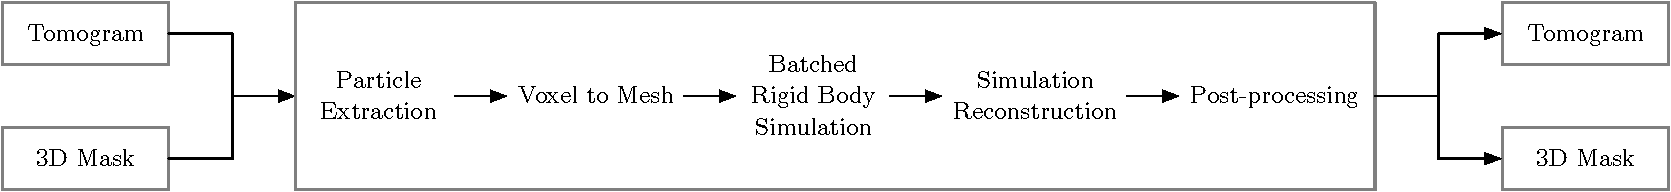
\includegraphics[width=\textwidth]{./figures/pdf/synthesis-workflow.pdf}
\end{figure}
\end{graphicalabstract}

%%Research highlights
\begin{highlights}
    \item We introduced a novel workflow that generates synthetic tomograms with segmentation ground truths. This method enriches existing tomographic datasets, offering capabilities for dataset augmentation and the evaluation of geological segmentation model.
\end{highlights}

\begin{keyword}
%% keywords here, in the form: keyword \sep keyword
Computed Tomography \sep Synthetic Data Generation
%% PACS codes here, in the form: \PACS code \sep code
% \PACS 0000 \sep 1111
%% MSC codes here, in the form: \MSC code \sep code
%% or \MSC[2008] code \sep code (2000 is the default)
% \MSC 0000 \sep 1111
\end{keyword}

\end{frontmatter}

%% \linenumbers

%% main text
%%%%%%%%%%%%%%%%%%%%%%%%%%%%%%%%%%%%%%%%%%%%%%%%%%%%%%%%%%%%%%%%%%%%%%%%%%%%%%%%
%%%%%%%%%%%%%%%%%%%%%%%%%%%%%%%%%%%%%%%%%%%%%%%%%%%%%%%%%%%%%%%%%%%%%%%%%%%%%%%%
%%%%%%%%%%%%%%%%%%%%%%%%%%%%%%%%%%%%%%%%%%%%%%%%%%%%%%%%%%%%%%%%%%%%%%%%%%%%%%%%
\section{Introduction} \label{sec:introduction}
In the field of geology, the use of computed tomography (CT) to scan geological particle samples has become increasingly common, such as reservoir rocks \cite{VANGEET200025}, sandstones \cite{cnudde20123d} and ores \cite{warlo2021multi}.
CT scanning offers significant advantage of providing 3D non-destructive inspection of large batches of particle samples, often referred to as particle packs.
However, to perform comprehensive analyses of these particle packs, it is essential to accurately segment individual particles. 
This segmentation is crucial for examining specific attributes such as composition and physical properties.
However, obtaining such segmentation is often the bottleneck in the tomographic analysis pipeline.
\par
With the growing utilisation of machine-learning-based segmentation algorithms, the demand for particle datasets has significantly increased. 
A key challenge in this context is the acquisition of CT volumes along with their precise ground truth segmentations. 
However, obtaining tomograms requires complex processes, highly skilled technicians, and sophisticated equipment. % which are not only expensive to operate but also resource-intensive. 
Moreover, research groups focused on developing segmentation algorithms may lack access to such CT datasets. 
\par
Synthetic data have been extensively utilised for decades to enhance existing datasets and evaluate computer vision algorithms, providing segmentation ground truth for tasks like autonomous driving \citep{richter2016playingdatagroundtruth}. 
This involves generating data that closely resembles real samples in structure, distribution, and essential characteristics, but are computationally produced.
Simulation-based methods are widely employed for this purpose \citep{demelo2022nextgeneration}, leveraging computational models such as physics simulators or scene rendering engines to create synthetic data tailored to specific domains. 
These methods aim to replicate real-world scenarios or physical phenomena by constructing virtual environments that mimic real-world dynamics with high fidelity.
Nevertheless, there is a lack of research on synthesising particle pack tomograms and their corresponding segmentations.
\par
In this work, we present a novel physics-simulation based workflow for generating 3D particle pack tomograms along with their corresponding segmentation ground truths. 
This approach provides an effective tool for augmenting tomographic segmentation datasets to enhance the training of machine learning-based segmentation models.
Furthermore, the synthesised dataset serves as a reliable benchmark for evaluating and validating segmentation algorithms.
\par
In this paper, we begin by introducing the workflow developed for synthesising particle pack datasets.
Next, we present experiments demonstrating how these datasets can augment segmentation model training, enhancing model performance.
Finally, we discuss the implications of our findings, highlighting their potential to improve segmentation accuracy and evaluation ability.

% \section{Background}
% talk in detail about literature review
% required theory to understand this paper
% successfully deployed tasks
% \par
% These simulation-based approaches have shown considerable success in various applications. 
% For instance, they are critical in generating annotated images for training object detection models in autonomous driving \citep{richter2016playing, abualhaija2018augmented}.
% \par
% pros and cons
% One of the main advantages of simulation-based methods is their high level of controllability \citep{muller2018sim4cv}.
% By allowing precise control over both the data generation process and the characteristics of the generated data, researchers and developers can ensure that the output closely adheres to specific criteria or regulatory requirements. 
% This transparency is crucial in understanding exactly how the data was produced, which is particularly beneficial in regulated industries where proving data integrity and compliance is essential. 
% Additionally, simulation-based methods are advantageous because they do not necessarily require large initial datasets. 
% Unlike methods that rely heavily on existing large volumes of data, simulations can generate valuable synthetic data from theoretical models or smaller existing datasets. 
% This capability is particularly useful in scenarios where real data is scarce or difficult to obtain.
% \par
% However, simulation-based methods have disadvantages.
% The complexity of creating accurate simulations represents a significant challenge \citep{demelo2022nextgeneration}; it is often a complex and time-consuming process that demands a thorough understanding of the underlying physical or logical processes that the data aims to represent. 
% Such complexity can limit the speed and scalability of data generation initiatives.
% Moreover, the novelty of data produced by simulation-based methods is inherently limited by the assumptions and rules embedded within the simulation data and models. 
% As a result, these methods might restrict the ability to uncover unexpected patterns or anomalies within the data, potentially leading to insights that are biased towards pre-conceived notions encoded in the simulation framework. 
% This limitation is particularly relevant in fields where discovering novel insights and understanding previously unrecognised phenomena are the primary objectives.

%%%%%%%%%%%%%%%%%%%%%%%%%%%%%%%%%%%%%%%%%%%%%%%%%%%%%%%%%%%%%%%%%%%%%%%%%%%%%%%%
%%%%%%%%%%%%%%%%%%%%%%%%%%%%%%%%%%%%%%%%%%%%%%%%%%%%%%%%%%%%%%%%%%%%%%%%%%%%%%%%
%%%%%%%%%%%%%%%%%%%%%%%%%%%%%%%%%%%%%%%%%%%%%%%%%%%%%%%%%%%%%%%%%%%%%%%%%%%%%%%%
\section{Method}\label{sec:method}
\begin{figure}
    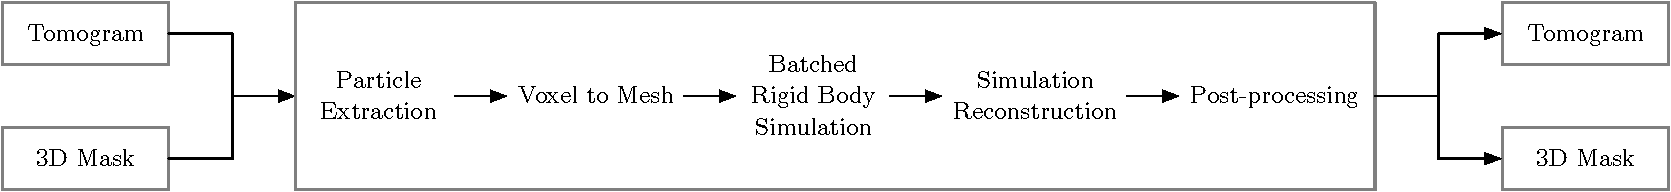
\includegraphics[width=\textwidth]{figures/pdf/synthesis-workflow.pdf}
    \caption{Particle Pack Synthesis Workflow}
    \label{fig:workflow}
\end{figure}
To illustrate our proposed workflow for generating synthetic particle packs (depicted in \Cref{fig:workflow}), we designed a process that closely replicates the physical steps involved in preparing particles for CT scanning. This workflow encompasses four key stages:
1. Mesh Acquisition, %: Extract particles from a CT-scanned particle pack volume and convert them into meshes.
2. Physical Simulation, %: Conduct rigid body simulations on the particle meshes using a physics simulator to obtain their rotations and positions in the simulated tomogram.
3. Synthetic Tomogram Creation, %: Create a synthetic particle pack tomogram and its 3D mask by combining the original particle volumes, masks, and simulation results.
4. Post-Processing.%: Introduce modifications, such as noise, to make the synthetic tomograms and masks realistic proxies for real-world data.

%===============================================================================
\subsection{Mesh Acquisition}
Mesh acquisition involves extracting each particle's volume from a tomogram and converting it into a mesh for rigid body simulations. 
As illustrated in \Cref{fig:mesh_acquisition_workflow}, the process starts with a particle pack tomogram and its mask. 
Using the mask, we isolate each particle's volume and label volume, then convert these into mesh format with marching cubes algorithm \citep{lorensen1987marching}.
To optimise for simulations, particle meshes can be simplified using mesh decimation techniques \citep{garland1997surface}. 
This reduces vertex counts while retaining essential geometry and improving simulation efficiency.
\begin{figure}[h!]
    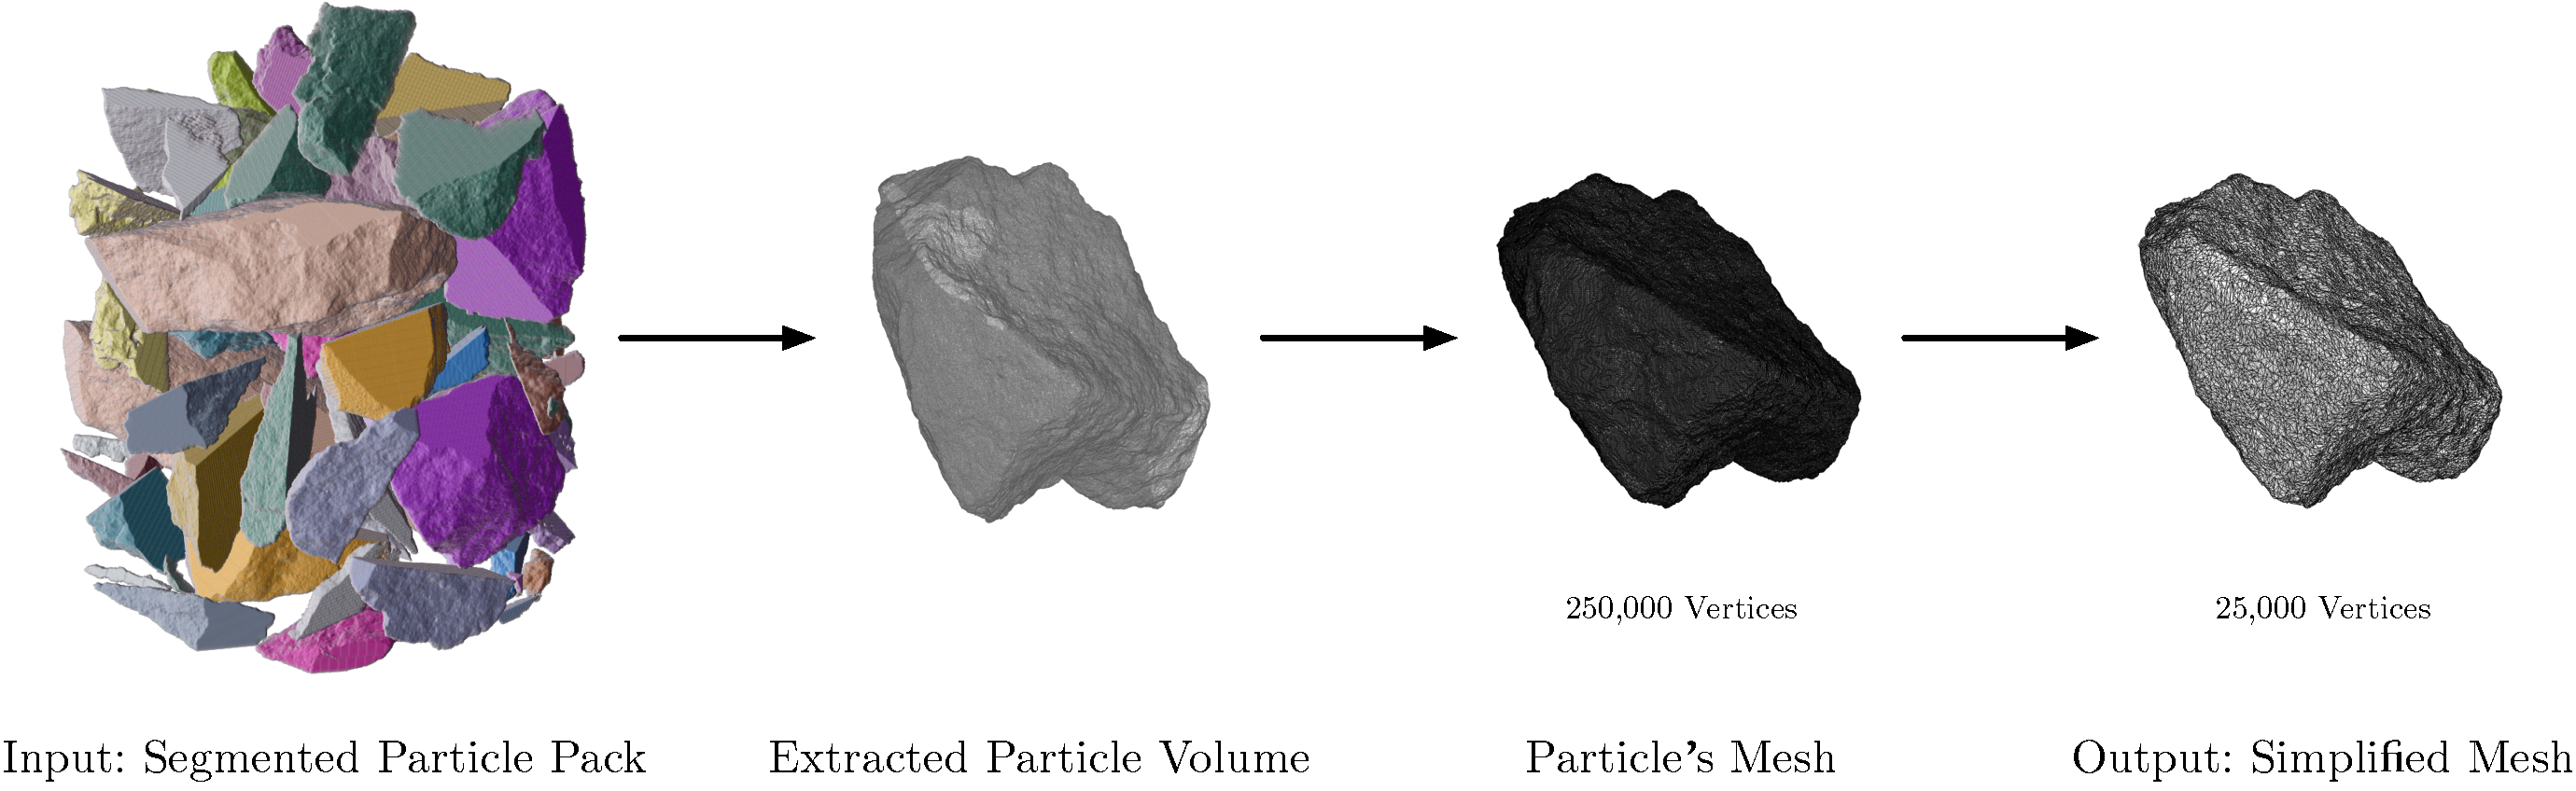
\includegraphics[width=\textwidth]{figures/pdf/mesh-acquisition.pdf}
    \caption{Mesh Acquisition Workflow}
    \label{fig:mesh_acquisition_workflow}
\end{figure}
%===============================================================================
\subsection{Physical Simulation}
The physical particle packing process begins with sieving to separate particles by size. 
Selected particles are then placed into a container to form a particle pack, ready for CT scanning.
Our goal in the physical simulation is to replicate this process.
This is achieved by inputting particle meshes with specific size then using a simulator to mimic the particle placement process, i.e., pouring particles into a container. 
Lastly obtain the placement (location and rotation) of each particle in the simulated particle pack.
\begin{figure}[H]
    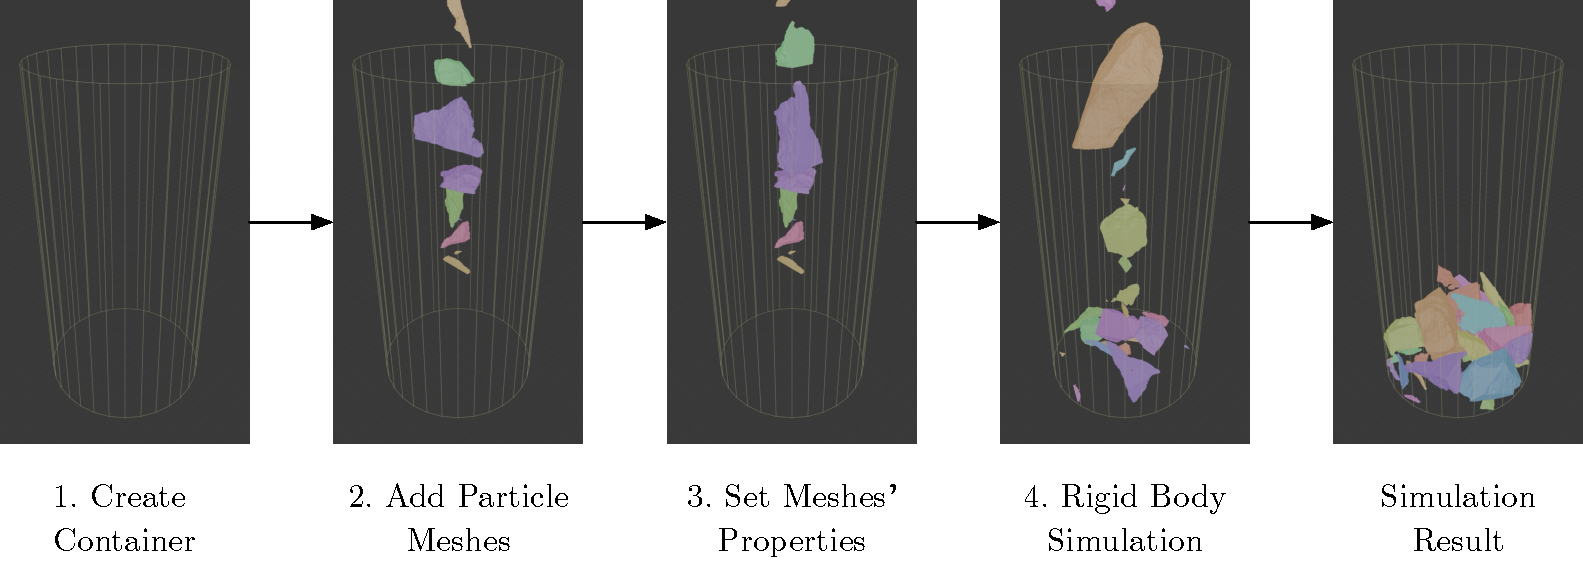
\includegraphics[width=\textwidth]{figures/pdf/simulation-pipeline.pdf}
    \caption{Pipeline of Batched Rigid Body Simulation}
    \label{fig:batched_rigid_body_simulation_pipeline}
\end{figure}
\par
The batched rigid body simulation pipeline includes four steps (illustrated in \Cref{fig:batched_rigid_body_simulation_pipeline}): 
\begin{enumerate}
    \item Create Container: Construct a tube-like container, similar to the one used in CT scans.
    \item Add Particle Meshes: Introduce particle meshes into the simulation environment.
    \item Set Meshes' Properties: Assign each particle mesh properties such as weight, initial position, and scale.
    \item Rigid Body Simulation: Start the simulation and allow the particle meshes to settle after a defined number of timesteps. The simulator will then output the final results, which contains each mesh's translation and rotation.
    Rigid body simulation is used to model this process because it approximates the motion and interaction of particles under realistic conditions, capturing essential dynamics such as collision, gravity, and friction without deforming the individual meshes.
\end{enumerate}
\par
After evaluating multiple options, including Unity 3D \citep{unity2024unity}, Unreal Engine \citep{unreal2024epic}, and PhysX \citep{nvidia2024nvidia}, we chose Blender \citep{blender2023objectops} for conducting batched rigid body simulations. 
Blender stood out due to its accessible graphical user interface (GUI), which facilitated the visual inspection of packed particle formations. 
This helped us verify whether the simulation accurately represents the desired physical characteristics.
Additionally, Blender's scripting interface allowed seamless integration into a Python-driven pipeline, ensuring that the project maintained a consistent and adaptable programming environment.
\par
In simulation of the particle packing processes, specific settings and procedures are crucial to achieving accurate and reproducible results. 
The implementation specifics used in our simulations include:
\begin{itemize}
    \item
    Particle weights affects collision between particles and container in our particle packing simulation. 
    In our implementation, we assume each particle has a uniformity and even quality. 
    Then the mass of each particle is estimated based on particles' density and the size of the particle.
    This method provides a rapid approximation of weight, suitable for scenarios where detailed precision is less critical. 
    \item
    The initial positioning and scaling of particle meshes are highly dependent on the experimental needs. 
    These adjustments significantly affect the final placement of particles within the volume. 
\end{itemize}
%===============================================================================
\subsection{Synthetic Tomogram Creation}
Based on the simulation results and particle volumes, the synthetic particle pack can be created. 
From the output of the simulation (step 3.2), we have a list of particle positions and orientations (rotations).
We also have the volumetric data of each particle from step 3.1. 
Given this, the synthetic tomogram creation is straightforward and involves three steps:
\begin{enumerate}
    \item Creating the target simulation container
    \item Rotating each particle volume according to the simulation results
    \item Placing each rotated particle volume in the simulation container based on the physics simulation results form 3.2
\end{enumerate}
%===============================================================================
\subsection{Post-processing}
Post-processing plays a crucial role in bridging the gap between synthetic and real-world data, enhancing the realism of synthetic tomograms. 
In our implementation, Gaussian noise is commonly added to replicate real-world imperfections, thereby producing a more realistic synthetic dataset.
Other artefacts can also be included, such as motion blur, ring effects, or beam hardening, which are common in tomographic imaging. 
By simulating these artefacts, synthetic datasets can closely mimic the challenges faced when processing real-world data, providing an invaluable ground truth for developing algorithms that are robust to these artefacts.
\par
An example of the post-processed synthesised slice is shown in \Cref{fig:syn:postprocess}. 
After post-processing, the synthetic slice appears more realistic.
\begin{figure}[H]
    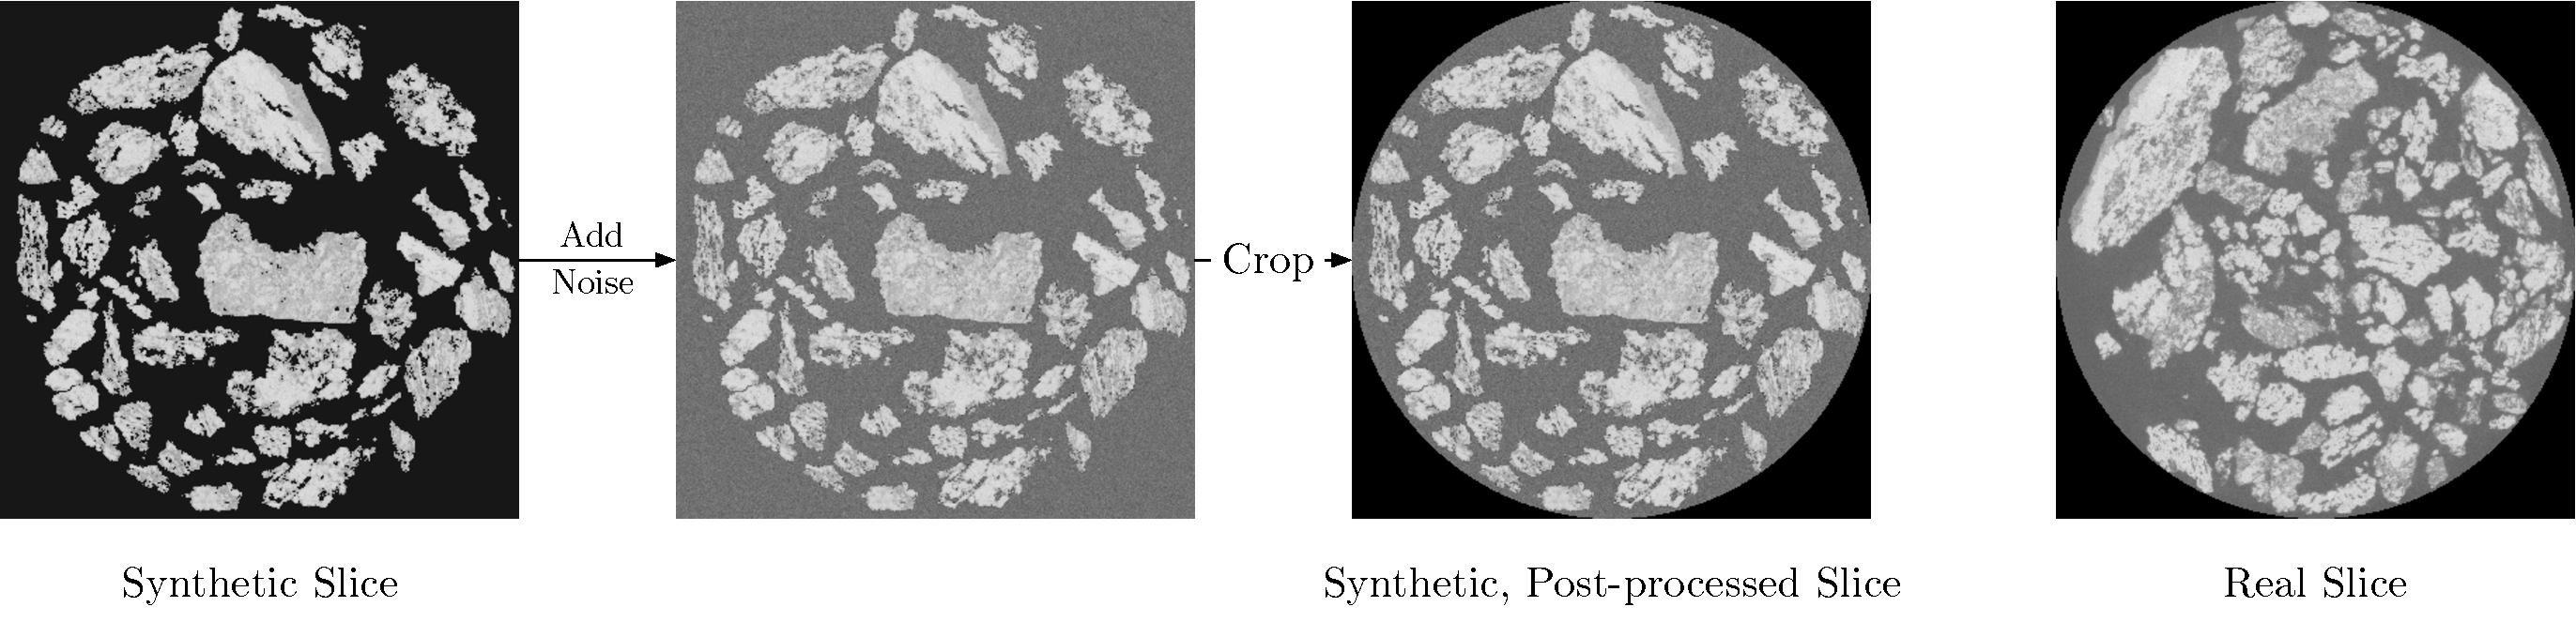
\includegraphics[width=\textwidth]{figures/pdf/postprocess.pdf}
    \caption{An Example of Postprocessing Slice in Simulated Particle Pack Data}
    \label{fig:syn:postprocess}
\end{figure}

\section{Experiment}
Having constructed synthetic particle packs as described in \Cref{sec:method}. 
We are therefore interested in investigating the efficacy of using synthetic particle packs to augment existing training datasets for particle pack segmentation.
This will be exemplified by comparing the performance gap between models trained on the original and augmented datasets.
% because we want to understand if using synthetic dataset can augment existing dataset therefore 
%===============================================================================
\subsection{Experiment Setup}
% whats the task (2d seg): intro, task, target
% why this task (2d seg): important as it's the cornerstone for subsequent analysis task 
% what tool do you use to seg: yolov8 (intro)
% why do you choose yolov8 (versatility)
% what evaluation metric do you use?
In this experiment, we investigate whether augmenting an existing dataset with synthetic data improves the performance of machine learning models trained for segmenting 2D particle packs. 
The segmentation target is illustrated in \cref{fig:syn:seg_target}. Given a 2D slice from a particle pack tomogram, the model aims to identify the background and individual particles, labelling each one distinctly.
\begin{figure}[H]
    \centering
    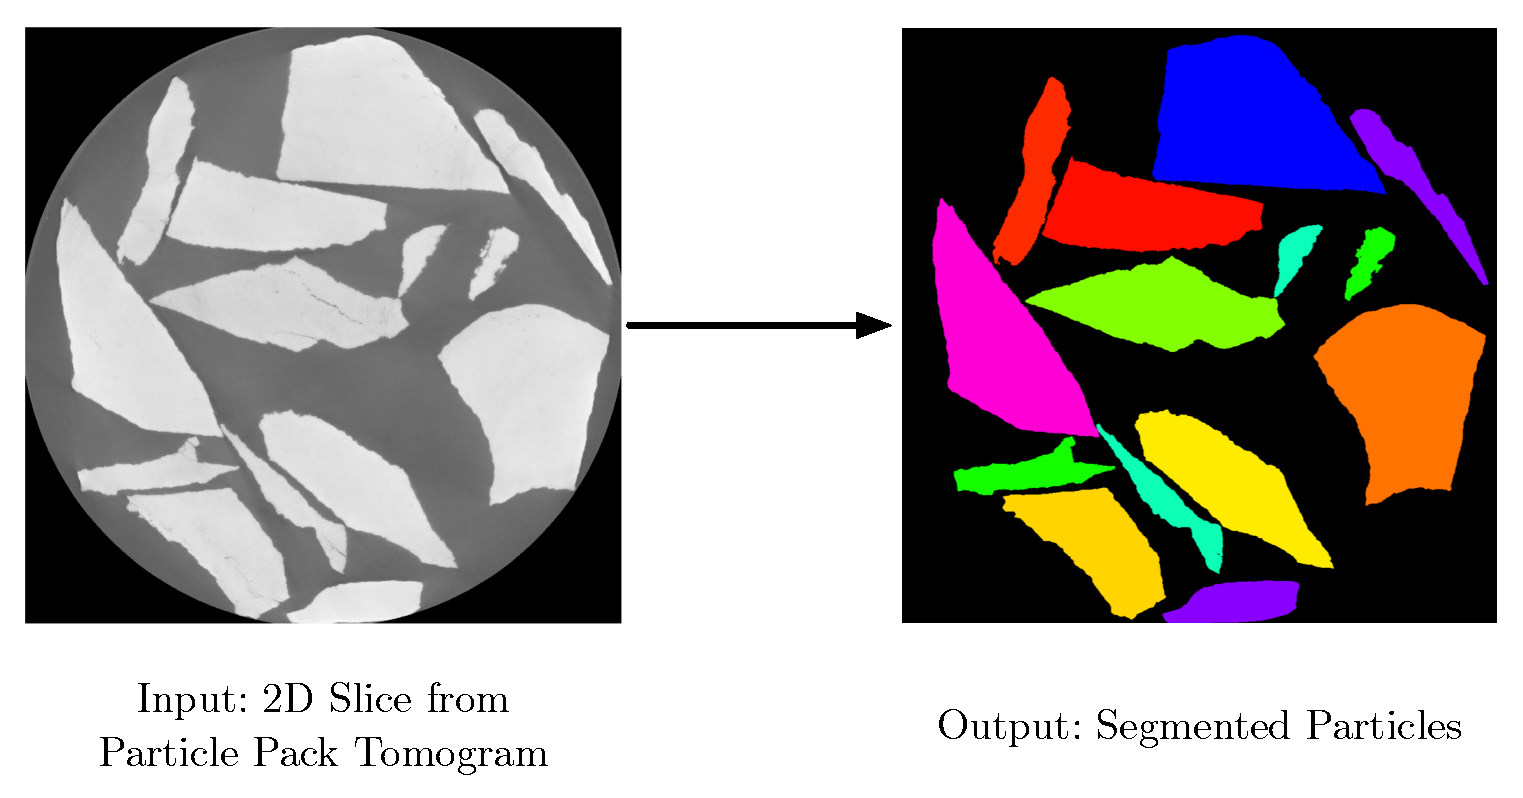
\includegraphics[width=0.7\textwidth]{figures/img/segmentation-intro.eps}
    \caption{An Illustration of 2D Particle Pack Segmentation}
    \label{fig:syn:seg_target}
\end{figure}
This experiment is motivated by two key factors: segmenting 2D particle packs is a challenging yet crucial task for subsequent analysis, and machine learning models for segmentation are increasingly prevalent but often face limitations due to a lack of high-quality training datasets.
\par
For segmentation, we utilise the YOLOv8 model developed by Ultralytics \citep{jocher2023yolo}.
YOLOv8 is a convolutional neural network (CNN) designed for efficient object detection and segmentation.
Specifically, the Yolov8m-seg variant is employed for this experiment for its versatility across diverse applications and its balance between computational efficiency and segmentation accuracy.
\par
To evaluate segmentation performance, we benchmark the number of correctly segmented pixels by comparing the model's output with the ground truth.
Thus Dice score \cite{Dice1945MeasuresOT}, also known as Dice-Sørensen coefficient, is particularly suitable for this purpose and is defined in \cref{eqn:dice}.
\begin{align}
    \label{eqn:dice}
    \text{Dice Score} = 2 \times \frac{\text{Area of Overlap}}{\text{Total Area}} 
    = \frac{
        2 \times \tikz[baseline=-.1cm]{
        \begin{scope}
            \fill[CarnationPink] (0,0) circle (0.5);
            \fill[CornflowerBlue] (0.5,0) circle (0.5);
            \clip (0,0) circle (0.5);
            \fill[Orchid] (0.5,0) circle (0.5);
            \fill[pattern=north east lines] (0.5,0) circle (0.5);
          \end{scope}
          \draw[line width=1pt, CarnationPink] (0,0) circle (0.5);
          \draw[line width=1pt, CornflowerBlue] (0.5,0) circle (0.5);
    }}
    {
        \tikz[baseline=-.1cm]{
            \begin{scope}
                \fill[CarnationPink] (0.0,0) circle (0.5);
                \fill[pattern=north east lines] (0.0,0) circle (0.5);
              \end{scope}
              \draw[line width=1pt, CarnationPink] (0,0) circle (0.5);
            }
            +
         \tikz[baseline=-.1cm]{
            \begin{scope}
                \fill[CornflowerBlue] (0.5,0) circle (0.5);
                \fill[pattern=north east lines] (0.5,0) circle (0.5);
              \end{scope}
              \draw[line width=1pt, CornflowerBlue] (0.5,0) circle (0.5);
            }
    }
\end{align}
%===============================================================================
\subsection{Iron Ore Dataset}
In this experiment, the baseline dataset used for training machine learning models is an iron ore dataset.
The dataset consists of a 3D tomogram, containing $x$ particles and $y$ slices, with each slice having dimensions of $2000 \times 2000$ pixels. (The values for $x$ and $y$ will be collected when I can access to Gadi.)
\par
To effectively train and evaluate our model, we partitioned the iron ore tomogram into training and testing sets. 
We specifically avoided random selection of slices for the testing set due to the high similarity between consecutive slices within the particle pack. 
This similarity can lead to overestimation of model performance, as the model might simply be recognising similar instances it has already encountered in adjacent slices, rather than generalising from diverse examples. 
Therefore, we allocated the central 20\% of the particle pack slices to the testing set, and the remaining 80\% for training.
\par
When utilising convolutional neural networks (CNNs) for segmentation, model performance can vary depending on the scale of objects. 
Therefore, for both the training and testing datasets, each 2D particle is classified as either small or large based on the dataset's median particle size.
%===============================================================================
\subsection{Synthetic Iron Ore Dataset}
The synthetic iron ore dataset was generated using our method, utilising the particles within the training set of the iron ore dataset described above. 
Additionally, the creation of the synthetic iron ore dataset involves post-processing to enhance realism. 
Gaussian noise is added to the synthetic tomogram to better mimic the characteristics of real-world data.
\par
The synthesised tomogram dataset contains $x$ particles and $y$ slices, with each slice having dimensions of $2000 \times 2000$ pixels. (The values for $x$ and $y$ will be collected when I can access to Gadi.) 
% A demonstration of the synthetic iron ore dataset is presented in \Cref{fig:syn:syn_dataset_examples}.
% \begin{figure}[]
%     \centering
%     \includegraphics[width=0.8\textwidth]{example-image-b}
%     \caption{Randomly sampled images from Synthetic Iron Ore Dataset}
%     \label{fig:syn:syn_dataset_examples}
% \end{figure}
%===============================================================================
\section{Results \& Analysis}
\begin{table}[]
    \center
    \begin{tabular}{|l|c|l|l|}
        \hline
                               & Post-processing & Real Large & Real Small \\ \hline
        Real Large             & n/a    & 94.5\%     & 77.0\%     \\ \hline
        Real Large + Syn       & \xmark & 94.9\%     & 79.6\%     \\ \hline
        Real Large + Syn       & \cmark & 96.0\%     & 80.1\%     \\ \hline \hline
        Real Small             & n/a    & 92.4\%     & 90.1\%     \\ \hline
        Real Small + Syn       & \xmark & 92.4\%     & 88.8\%     \\ \hline
        Real Small + Syn       & \cmark & 94.8\%     & 90.9\%     \\ \hline
    \end{tabular}
    \caption{Segmentation performance between models trained on different datasets. 
    Each row represents the training set, and each column represents the testing set (except for the ``Post-processing'' column). 
    The ``Post-processing'' column indicates whether the augmented dataset has been post-processed.
    Real Large refers to a real tomogram dataset with large particles, while Real Small refers to a real tomogram dataset with small particles. 
    Rows include results from training on only the real datasets and combinations with synthetic data (Real Large + Syn, Real Small + Syn). 
    Columns indicate testing on real datasets with large or small particles.
    }
    \label{tab:res1}
\end{table}
\subsection{Result I: Postprocessing Is Crucial In Augmentation}
The observed results from \Cref{tab:res1} indicate that after post-processing, the training dataset was successfully augmented, leading to improvements in the models' performance across various test sets. 
Conversely, without adding noise, the models' performance sometimes degraded (from 90.1\% to 88.8\%).
\par
This can be attributed to the noise making the synthetic slices more realistic and closer to the actual data the model will encounter, thereby reducing the domain gap between synthetic and real data.
Without noise, the synthetic data lacks the necessary realism, leading the model to learn features that do not transfer well to real-world scenarios.
This discrepancy can cause the model to perform poorly on real data, effectively learning in a different domain than the one it is tested on. This highlights the importance of appropriate postprocessing to make synthetic datasets more realistic, which enhances its utility for augmenting existing datasets.
%===============================================================================
\subsection{Result II: Synthetic Data Improves Segmentation Accuracy}
To assess performance improvements with synthetic particle packs, we trained and tested segmentation models using real data alone, and real data augmented with synthetic particle pack data. 
The results for each model, presented in \Cref{tab:res1}, demonstrate that incorporating synthetic data improves segmentation performance under most scenarios.
Specifically, when trained with real large particles augmented with synthetic data, the accuracy increased from 94.5\% to 96.0\% for large particles and from 92.4\% to 94.8\% for small particles. 
Similarly, training with real small particles combined with synthetic data improved the accuracy on large particles from 77.0\% to 80.1\%, while the improvement for small particles was more modest, rising from 90.1\% to 90.9\%. 
These results indicate that synthetic data enriches the training set with diverse examples, thereby enhances the model's ability to segment tomograms with different particle sizes. 

\section{Discussion}
The findings of this study underscore the potential of synthetic data augmentation in enhancing the segmentation accuracy of machine learning models applied to 2D particle pack datasets. 
Notably, the results demonstrate significant improvements in Dice scores when synthetic datasets are incorporated into the model training process. 
These improvements were particularly pronounced in the segmentation of large particles, suggesting that the augmented dataset effectively enriches the diversity of training examples, thereby enhancing the model's ability to generalise.
\par
Furthermore, we also demonstrated that post-processing techniques such as Gaussian noise plays a critical role of enhancing realism in synthetic datasets for model training. 
Post-processing reduces the domain gap between synthetic and real-world data, enabling the model to learn more transferable features.
\par
Our method also demonstrate its potential in, firstly, offering an effective tool for augmenting tomographic segmentation datasets, enhancing model training through increased data diversity;
Secondly, these datasets serve as a reliable resource for evaluating and validating segmentation models. 
Unlike manually created ground truth data, which may contains artefacts in tomogram or incorrect labelling, the synthesised dataset can be generated without flaws. 
This ensures greater accuracy and consistency, enabling robust model evaluation and validation.
\par
The current synthetic particle pack generation workflow is constrained by its reliance on manually labelled particle packs. 
This limitation reduces the particles' versatility in the generated particle packs. 
To eliminate this dependency and increase data diversity, we propose two improvement directions. 
The first approach involves using methods such as free-form deformation (FFD) \cite{sederberg1986free} to alter particles' shape while retaining their core characteristics.
This method is relatively fast, easy, and deterministic but still relies on the existing particle data.
The second approach involves employing advanced machine-learning techniques, such as diffusion models \cite{ho2020denoising} or generative adversarial networks (GANs) \cite{goodfellow2014generativea}. 
These models would first learn the features of the particle data and then generate entirely synthetic particle data. 

% Ideas: 
% \begin{itemize}
%     \item Findings: how our work improves segmentation? Importance of postprocessing
%     \item Limitations: requires existing particle packs, computational complexity in simulation and tomogram creation?
%     \item Practical implications: how can we support for future research?
%     \item using it for testing: 1. size, 2. provide ground truth in large quantity (many ground truth)
%     % describe the experiment: experiment
%     % how much noise to add?
%     % mention add other artefacts
%     % list of things findings
%     % include some use cases / examples
%     % 1. create new dataset
%     % 2. extend existing
%     % 3. create dataset for testing / benchmarking
%     % Conclusion: do not include anything new in conclusion
% \end{itemize}

\section{Conclusion}
This paper presents a comprehensive workflow for generating synthetic particle pack datasets through physics-based simulation. 
Our approach addresses the challenges of acquiring accurate particle pack tomograms and segmentation ground truths in geology. 
These tomogram-mask pairs can be used to augment existing segmentation datasets and evaluating segmentation algorithms. 
The integration of noise and artefacts in post-processing further bridges the gap between synthetic and real-world data, offering a data generation platform for future research. 
\par
Our experimental results validate the effectiveness of our synthetic particle pack generation workflow. 
By augmenting real datasets with synthetic data, we achieved consistent improvements in segmentation accuracy across different particle sizes. 
The integration of post-processing techniques, specifically the addition of noise, was crucial in bridging the gap between synthetic and real-world data, leading to enhanced model performance. 
These findings highlight the potential of our approach to enrich annotated particle pack data for training and validation of segmentation algorithms.
% \par
% In the current synthetic particle-pack-generation workflow, we rely on manually labelled particle packs, which limits the versatility of the particle data. 
% To eliminate this dependency and increase data diversity, we propose two improvement directions. 
% The first approach involves using classical methods such as free-form deformation (FFD) \cite{sederberg1986free} to alter particles' shape while retaining their core characteristics. 
% This method is relatively fast, easy, and deterministic but still relies on the existing particle data.
% The second approach involves employing advanced machine-learning techniques, such as diffusion models \cite{ho2020denoising} or generative adversarial networks (GANs) \cite{goodfellow2014generativea}. 
% These models would first learn the features of the particle data and then generate entirely synthetic particle data. 
%% The Appendices part is started with the command \appendix;
%% appendix sections are then done as normal sections
% \appendix

% \section{Sample Appendix Section}
% \label{sec:sample:appendix}
% Lorem ipsum dolor sit amet, consectetur adipiscing elit, sed do eiusmod tempor section \ref{sec:introduction} incididunt ut labore et dolore magna aliqua. Ut enim ad minim veniam, quis nostrud exercitation ullamco laboris nisi ut aliquip ex ea commodo consequat. Duis aute irure dolor in reprehenderit in voluptate velit esse cillum dolore eu fugiat nulla pariatur. Excepteur sint occaecat cupidatat non proident, sunt in culpa qui officia deserunt mollit anim id est laborum.

%% If you have bibdatabase file and want bibtex to generate the
%% bibitems, please use
%%
 \bibliographystyle{elsarticle-num} 
 \bibliography{cas-refs}

%% else use the following coding to input the bibitems directly in the
%% TeX file.

% \begin{thebibliography}{00}

% %% \bibitem{label}
% %% Text of bibliographic item

% \bibitem{}

% \end{thebibliography}
\end{document}
\endinput
%%
%% End of file `elsarticle-template-num.tex'.
